% !TeX root = main.tex
% Answer to Question 1 (Version 1)

\section{Q1: Keypoint Detection and Description}

\paragraph*{Question}
\begin{displayquote}
    % !TeX root = main.tex
\section{Basics of Optical Flow}

\subsection{Thought Experiments}

\subsubsection{Bullet Time - The Matrix (1999)}

\paragraph*{Question}
Explaining how optical flow is used for the \href{https://www.youtube.com/watch?v=8DajVKAkL50}{bullet time scene} in The Matrix (1999).

\paragraph*{TL; DR}
Frame interpolation using optical flow.

\paragraph*{Full Answer}
A series of cameras are arranged in the scene, starting from the point where the scene starts (in perspective view) and till the end. For this scene in particular, 120 cameras were used (watch reference video \href{https://youtube.com/clip/UgkxKwMsGJCjo-0t9dnsaD6vtVRMl-JRj4wv}{here} \footnote[1]{\url{https://filmschoolrejects.com/the-matrix-bullet-time/}}).

The actor is put in a green screen environment, at the center of those cameras. The action is performed at normal speed (human speed), with the cameras capturing the sequence with a slight time delay. Say the scene (the complete pose change of Neo) takes 1 second, but in the final movie, it is 10 seconds. Let's assume that the movie is 25 FPS and that the 120 camera captures are equally spaced in the entire band. That is, dividing $25\times 10 = 250$ frames into $120$ cameras giving approximately one real image (taken by the camera) followed by one interpolated image.

The problem now becomes finding the interpolated images. Theoretically, repeating the real image will create a jittery motion (it will seem to lag). The intermediate image can be estimated through \emph{optical flow}. Since Neo (actor Keanu Charles Reeves) is on a green screen, tracking motion is relatively easier. For two real image captures given, the pixels of the intermediate frame is the half-displacement applied to each pixel. The total displacement is estimated through optical flow.

\subsubsection{Painterly rendering - WDMC (1998)}

\paragraph*{Question}
Explaining the \href{https://www.youtube.com/watch?v=CYonzhFT_z4}{painterly effect scene} in What Dreams May Come (1998).

\paragraph*{TL; DR}
Transformation and tracking of particles are done using optical flow.

\paragraph*{Full Answer}

Interestingly, the scene was probably captured using the work of Barbara Meier (Senior Lecturer at Brown University) in \cite{meier1996painterly} \footnote[6]{Source: \href{https://news.brown.edu/new-faculty/physical-sciences/barbara-meier}{news.brown.edu}}. The painterly rendering pipeline uses the geometry of the object being painted (usually a triangle mesh). It gets particles (samples) in world space. Shaders are used to extract the \textbf{color} (color attributes and lighting), \textbf{size} (lighting, texture map and user-specified paintbrush attributes) and \textbf{orientation} (surface normal projection). A \emph{brush image} showing the texture of the brush pattern is used. 

Brush strokes are made on a canvas based on the attributes (emphasized above). These brush strokes are applied to the particles. In an animation, to maintain consistency, it is important to track these particles and use only them. Optical flow yields estimates of where the particles flow in successive frames. It can also be used to save computation by rearranging geometry using optical flow (the above-described process is computation heavy). An example application was developed as a project in \href{https://www.dgp.toronto.edu/~mccrae/projects/paintanimation/#:~:text=The%20project%20allows%20one%20to,temporal%20artifacts%20can%20be%20produced}{DGP Toronto}.

At the time the movie was developed, they must have chosen many properties by hand. Later developments in the field alleviate this load and make things much easier \cite{painterly-animation-1, painterly-animation-2,painterly-animation-3}.

\subsubsection{Lambertian ball}

Assuming that the Lambertian ball doesn't have any features or texture on its surface (as is usually the case) and only reflects light (to create visual features).

\paragraph*{Lighting fixed, ball rotating}

In the case where lighting is fixed, and the ball is rotating, \emph{we will probably not get any optical flow} features out of it. This is because the ball has no texture, and since the lighting is fixed, the visual appearance (because of reflection) will remain the same. So the individual pixels will probably not change their values much, and hence there won't be any optical flow. This is nicely demonstrated in \href{https://www.youtube.com/clip/UgkxbMT3LuFK5px5D2Uczx2lduW3QQW9_3YD}{this clip} where even the human would find it hard to recognize that the ball is rotating. This can be seen in Figure \ref{fig:q1-lambertian-ball}.

\begin{figure}[h]
    \centering
    \begin{subfigure}[b]{0.25\textwidth}
        \centering
        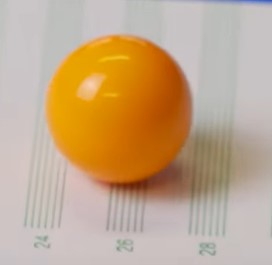
\includegraphics[width=\textwidth]{Lambertian_ball_0_13.jpg}
        \caption{0:13}
    \end{subfigure}
    \begin{subfigure}[b]{0.25\textwidth}
        \centering
        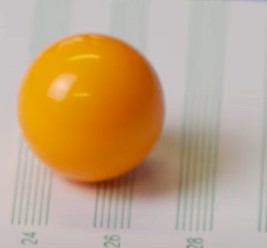
\includegraphics[width=\textwidth]{Lambertian_ball_0_15.jpg}
        \caption{0:15}
    \end{subfigure}
    \caption{Rotating Lambertian ball}
    \label{fig:q1-lambertian-ball}
    \small
        The two images are taken at different timestamps \href{https://www.youtube.com/clip/UgkxbMT3LuFK5px5D2Uczx2lduW3QQW9_3YD}{in the clip}. The orange ball is rotating, but it can't clearly be said from looking at the two images.
\end{figure}

\paragraph*{Lighting moves, ball fixed}

In the case where the ball is fixed, and the lighting is moved, \emph{we will see the optical flow on the ball's surface}. This is because the reflection of the lighting will move on the ball's surface, which means that the pixels on the ball will appear to move. This can be seen in 

\begin{figure}[h]
    \centering
    \begin{subfigure}[b]{0.25\textwidth}
        \centering
        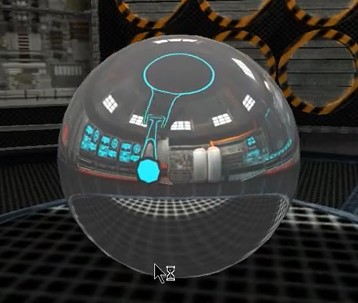
\includegraphics[width=\textwidth]{Lambertian_ball_light_2_41.jpg}
        \caption{Pose 1}
        \label{fig:sfig-q1-ball-lighting-1}
    \end{subfigure}
    \begin{subfigure}[b]{0.25\textwidth}
        \centering
        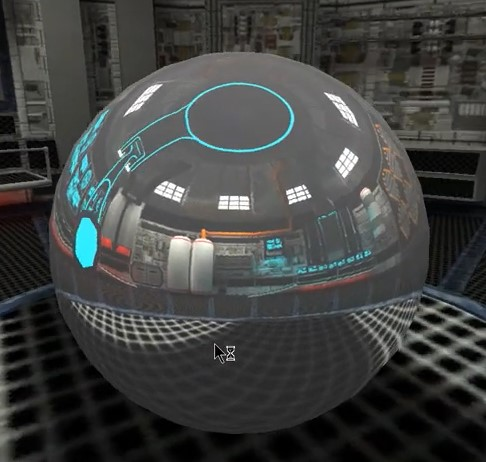
\includegraphics[width=\textwidth]{Lambertian_ball_light_2_43.jpg}
        \caption{Pose 2}
        \label{fig:sfig-q1-ball-lighting-2}
    \end{subfigure}
    \caption{Illumination moving}
    \label{fig:ball-lighting-}
    \small
        The two poses of the blue light are different on the ball. This gives a virtue of motion to the texture. 
        
        Images are from \href{https://www.youtube.com/watch?v=_pK4Rkprj2Q}{UserBenchmark tests on YouTube}, figure \ref{sub@fig:sfig-q1-ball-lighting-1} from \texttt{2:41} and \ref{sub@fig:sfig-q1-ball-lighting-2} from \texttt{2:43}.
\end{figure}

\subsection{Concept Review}
\label{sec:q1-concept-review}

Optical flow aims to recover pixel-level motion between two images.

\noindent
Some references for Optical Flow (not for reviewers)

\begin{itemize}
    \item \href{https://www.youtube.com/watch?v=5AUypv5BNbI}{YouTube: Optical Flow - Computerphile}
    \item \href{https://www.youtube.com/watch?v=4v_keMNROv4}{YouTube: Optic Flow Solutions - Computerphile}
\end{itemize}

\subsubsection{Assumptions of Optical Flow}

Some key assumptions in optical flow are as follows

\begin{itemize}
    \item \textbf{Brightness consistency} assumption: The brightness of a particular pixel (after being moved to a new pixel) is the same. That is, $I(x, y, t) = I(x+u, y+v, t+1)$.
    \item \textbf{Spatial Coherence constraint}: Assume that the neighbors of the pixel being inspected have the same motion. That is, the blob has the same displacement. This allows us to solve the problem as a least-squares problem. This was first introduced in \cite{lucas1981iterative}.
    \item It is also assumed that there is no change in environment illumination and only a small motion has occurred between the frames that are being analyzed.
\end{itemize}

\subsubsection{Objective function}

The problem of optical flow is to track the motion of pixels in the neighborhood, that maintain color consistency (we assume that they are the same pixels if they have the same color).

\begin{figure}[h]
    \centering
    \begin{subfigure}[b]{0.4\textwidth}
        \centering
        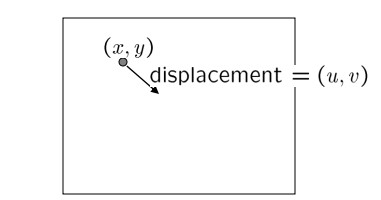
\includegraphics[width=\textwidth, height=6cm, keepaspectratio]{oflow_exp_im1.jpg}
        \caption{$t$}
    \end{subfigure}
    \begin{subfigure}[b]{0.4\textwidth}
        \centering
        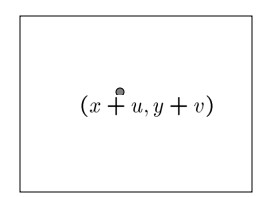
\includegraphics[width=\textwidth, height=3.375cm, keepaspectratio]{oflow_exp_im2.jpg}
        \caption{$t+\Delta t$}
    \end{subfigure}
    \caption{Pixel positions at different times}
    \label{fig:q1-opflow-fig}
    \small
        The pixel in the left image moves to the right image by $\sfrac{\Delta x}{\Delta t} = u$, $\sfrac{\Delta y}{\Delta t} = v$.
\end{figure}

\paragraph*{Brightness Consistency}

Applying the \emph{Brightness consistency} constraint to figure \ref{fig:q1-opflow-fig}, we get

\begin{align*}
    I(x+\Delta x, y+\Delta y, t+\Delta t) \approx I(x, y, t)
\end{align*}

The small motion assumption allows us to apply Taylor series expansion to the above equation

\begin{align}
    I(x+u, y+v, t+\Delta t) &= I(x, y, t) + \frac{\partial I}{\partial x} \Delta x + \frac{\partial I}{\partial y} \Delta y + \frac{\partial I}{\partial t} \Delta t + \textup{higher order terms}
    \nonumber \\
    &\approx I(x, y, t) + \frac{\partial I}{\partial x} \Delta x + \frac{\partial I}{\partial y} \Delta y + \frac{\partial I}{\partial t} \Delta t
    \label{}
\end{align}

Merging the above two equations, we get

\begin{align*}
    0 &\approx \frac{\partial I}{\partial x} \Delta x + \frac{\partial I}{\partial y} \Delta y + \frac{\partial I}{\partial t} \Delta t 
    &&
    \frac{\partial I}{\partial x} = I_x \quad
    \frac{\partial I}{\partial y} = I_y \quad
    \frac{\partial I}{\partial t} = I_t
    \\
    \Rightarrow 0 &= I_x \: \Delta x + I_y \: \Delta y + I_t \Delta t = \left[ I_x \;\; I_y \right] \cdot \left[ \Delta x \;\; \Delta y \right] + I_t \Delta t 
    &&
    \left[ I_x \;\; I_y \right] = \triangledown I
    \\
    & \Rightarrow \triangledown I \cdot \left[ u \;\; v \right] + I_t = 0
\end{align*}

The data terms (obtained through the image) and the spatial terms (algorithm finds these) are marked below

\begin{equation}
    \underbrace{\left[ I_x \;\; I_y \right]}_{\textup{data term}} \cdot \underbrace{\left[ u \;\; v \right]}_{\textup{spatial term}} + \underbrace{I_t}_{\textup{data term}} = 0
    \label{eq:q1-oflow-direct}
\end{equation}

\paragraph*{Generalized Implementation}
As implemented in \cite{lucas1981iterative}. Consider $F$ and $G$ as images and $\mathbf{x}$ as pixel position and $\mathbf{h}$ as the shift in position (possibly of a region $R$). We wist to minimize the $\textup{L}_2$ norm error

\begin{equation*}
    \textup{E}_{\textup{L2}} = \sum_{\textbf{x} \in R} \left[ F(\mathbf{x+h}) - G(\mathbf{x}) \right]^2
\end{equation*}

Using the taylor expansion

\begin{equation*}
    F(\mathbf{x+h}) = F(\mathbf{x}) + h_x \frac{\partial F}{\partial x} + h_y \frac{\partial F}{\partial y} = F(\mathbf{x}) + \mathbf{h} \frac{\partial F}{\partial \mathbf{x}}
\end{equation*}

To obtain the $\mathbf{h}$ that minimizes the error $\textup{E}_{\textup{L2}}$, we do the following

\begin{align*}
    0 &= \frac{\partial \textup{E}_{\textup{L2}}}{\partial \mathbf{h}} \\
      &= \frac{\partial }{\partial \mathbf{h}} \sum_{\textbf{x} \in R} \left[ F(\mathbf{x+h}) - G(\mathbf{x}) \right]^2 \\
    \frac{\partial E}{\partial h_x} &= \sum_{\textbf{x} \in R} \left [ F(\mathbf{x}) + h_x \left ( \frac{\partial F}{\partial x} \right )^2 + h_y \left ( \frac{\partial F}{\partial x} \right ) \left ( \frac{\partial F}{\partial y} \right ) - G(\mathbf{x}) \left ( \frac{\partial F}{\partial x} \right ) \right ] \\
    \frac{\partial E}{\partial h_y} &= \sum_{\textbf{x} \in R} \left [ F(\mathbf{x}) + h_x \left ( \frac{\partial F}{\partial x} \right ) \left ( \frac{\partial F}{\partial y} \right ) + h_y \left ( \frac{\partial F}{\partial y} \right )^2 - G(\mathbf{x}) \left ( \frac{\partial F}{\partial y} \right ) \right ]
\end{align*}

This gives the final equation

\begin{equation}
    \mathbf{h} = \begin{bmatrix} h_x & h_y \end{bmatrix} = \left [ \sum_{\mathbf{x} \in R} \begin{pmatrix}
        \frac{\partial F}{\partial x} & \frac{\partial F}{\partial y}
        \end{pmatrix} \left( G(\mathbf{x}) - F(\mathbf{x}) \right ) \right ] \begin{bmatrix}
        \sum_{\mathbf{x} \in R} \left ( \frac{\partial F}{\partial x} \right )^2 &
        \sum_{\mathbf{x} \in R} \left ( \frac{\partial F}{\partial x} \right ) \left ( \frac{\partial F}{\partial y} \right ) \\
        \sum_{\mathbf{x} \in R} \left ( \frac{\partial F}{\partial x} \right ) \left ( \frac{\partial F}{\partial y} \right ) &
        \sum_{\mathbf{x} \in R} \left ( \frac{\partial F}{\partial x} \right )^2
        \end{bmatrix}^{-1}
\end{equation}

The above equation has the data terms on the right hand side.

\subsubsection{Taylor series approximation}

It is assumed that the motion is small. This means that the second derivative will almost have no value throughout the image. Therefore, the displacement is assumed to be linearly approximated to the first derivative, in the Taylor expansion.

The first order approximation also makes the differentiation task easier, as seen when minimizing $\textup{E}_{\textup{L2}}$ with respect to $\mathbf{h}$.

Second order derivatives will involve calculating Laplacians and Hessians (which are more expensive).

\subsubsection{Ill-posed constraint}

The constraint of brightness consistency (borrowed from \cite{horn1981determining}) is given by

\begin{equation}
    I_x u + I_y v + I_t = 0 \Rightarrow \left ( I_x, I_y \right ) \cdot \left ( u, v \right ) = -I_t
\end{equation}

In such a case, optical flow perpendicular to the image gradient $I_x, I_y$ cannot be uniquely distinguished. This is demonstrated in the figure below.

\begin{figure}[h]
    \centering
    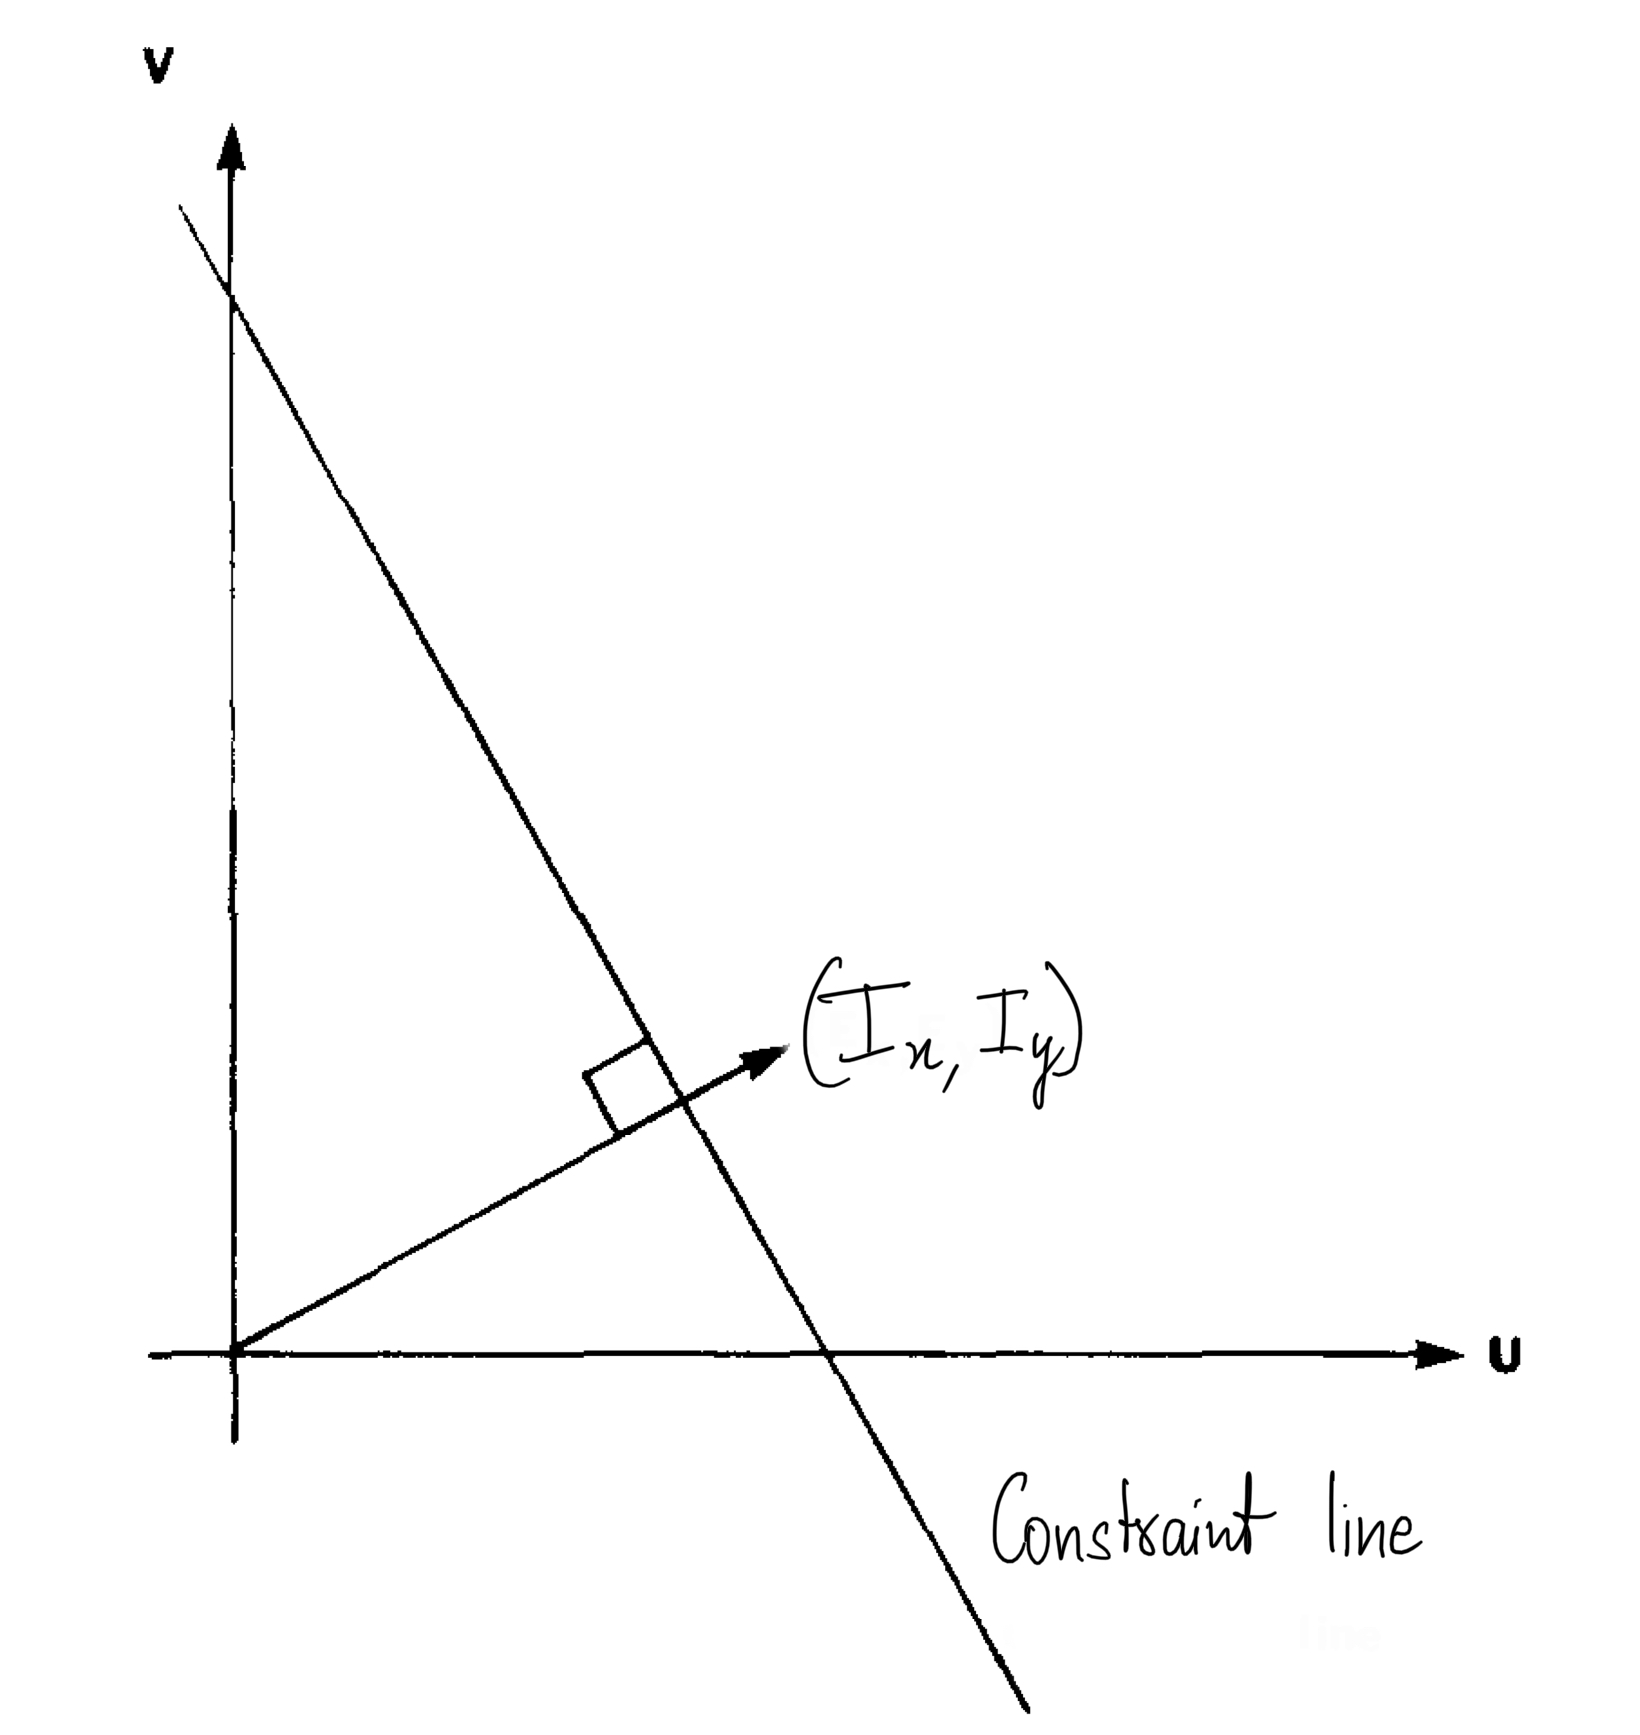
\includegraphics[width=0.4\textwidth]{opt_flow_constraint_ill_posed.PNG}
    \caption{Ill-posed optical flow constraint}
\end{figure}

\end{displayquote}

Keypoints are points of \emph{interest} and are useful in image matching and description. Keypoints have to be \emph{detected} (location found in an image) by a detector, and they have to be described by a \emph{descriptor} (for some unique identification).

The answer is described in the subsections below.

% SIFT
\subfile{q1_v1_sift.tex}

% SURF
\subfile{q1_v1_surf.tex}

% Ensemble
\subsection{Ensemble}

\paragraph*{TL; DR}
It depends on the application. Let us take the application of \emph{finding feature correspondences between two images} as an example.

\paragraph*{Example}

The aim is to match the identical features in two images. Feature description plays an essential role here.

Traditionally, the descriptors are uniquely defined for each method (SIFT and SURF, for Example, have different descriptor formats). They, therefore, cannot be concatenated or merged in any easy way. 

However, we can apply some tricks to get an ensemble of correspondences. One of them is to apply descriptor matching (using techniques like the mutual nearest neighbor, cosine distance, Euclidean distance, or Mahalanobis distance) for the \emph{individual} methods (separately). Then, obtain the keypoints (again, separately) and then concatenate the obtained keypoints. We now have point correspondences from both methods.

Such methods can boost correspondences between two images by a significant margin.
